\documentclass[12pt, A4Paper]{article}
\usepackage[utf8]{inputenc}
\usepackage{graphicx}
\usepackage{float}

\usepackage{color}   %May be necessary if you want to color links
\usepackage{hyperref}
\hypersetup{
    colorlinks=true, %set true if you want colored links
    linktoc=all,     %set to all if you want both sections and subsections linked
    linkcolor=blue,  %choose some color if you want links to stand out
}

\title{Snort Report}
\author{Fahad Ahmed Akash}
\date{March 2024}

\begin{document}

\begin{titlepage}
   \begin{center}

       \LARGE{\textbf{Computer Security Project Report}}

       \vspace{1cm}
       \Large{\textbf{CSE 406}}\\
       \vspace{0.5cm}
       \large{\textbf {Tool: John The Ripper}}
       
        \vspace{2cm}
    \textbf{Supervisor:}\\
       Abdur Rashid Tushar\\
       Lecturer\\
       CSE, BUET\\
       
       
      \vspace{3cm}
    \textbf{Presented By:}\\
       Rayan Islam - 1905106\\
       Fahad Ahmed Akash - 1905107
            
       \vspace{2cm}
        Level-4 Term-1\\
        Department of CSE\\
       Bangladesh University of Engineering \& Technology\\
       11 March, 2024\\
            
   \end{center}
\end{titlepage}



\tableofcontents

\newpage

\section{Introduction}
John the Ripper is a password cracking tool. The tool is used by security professionals to test the strength of passwords. It is very powerful and versatile. It employs various techniques such as brute-force attacks, dictionary attacks, and hybrid attacks to uncover weak passwords in different environments. Originally developed for Unix systems, it has since been ported to numerous platforms, making it widely accessible for security testing purposes.

\section{Tool Overview}
John the ripper is an open source password cracking tool. It is widely used for analysis of the strength of passwords. Here is an overview of John the ripper's key features and functionalities:


\begin{enumerate}
    \item \textbf{Multiple Hash Formats:} It supports numerous hash types, allowing it to crack passwords stored in various formats - 
    \begin{itemize}
        \item Windows LM hashes
        \item MD5
        \item SHA-1 etc.
    \end{itemize}
    Moreover, it uses a modular architecture, enabling users to add new hash types or cracking methods easily through plugins.

    \item \textbf{Multiple Attacks:} John the ripper allows the user to work in multiple modes, such as -

    \begin{enumerate}
        \item \textbf{Dictionary Attack}
        \begin{itemize}
            \item \textbf{Wordlist Mode:} This mode allows John to use a list of potential passwords (often derived from real words or common password choices) to attempt to crack the hash.
            \item \textbf{Brute Force and Incremental Mode:}  It can perform brute-force attacks, trying all possible combinations of characters up to a certain length, and incremental attacks, which systematically cover all possible plaintexts.
        \end{itemize}   
        \item \textbf{Rules-based Attack:}  This allows users to apply various modifications to wordlist entries (like capitalization, character replacement, or affixing numbers) to crack passwords that involve common substitutions or simple variations on dictionary words.
    \end{enumerate}

    \item \textbf{Parallel Processing:} It can take advantage of multiple CPUs and multi-core CPUs, along with certain GPUs, to increase cracking speed.es

    \item \textbf{Community-enhanced Versions:}  There are community-enhanced versions like John the Ripper Jumbo, which include additional features and support for many more hash types and cracking methods not found in the standard version.

    \item \textbf{Portability:} It runs on a variety of operating systems, including -  
    \begin{itemize}
        \item Unix
        \item Windows
        \item DOS
        \item BeOS
        \item OpenVMS
    \end{itemize}
\end{enumerate}
\vspace{0.4cm}

\section{Installation}
To install John the Ripper from its GitHub repository, follow these steps - 

\begin{itemize}
    \item {\textbf{Clone the repository:}} \newline
   git clone \href{https://github.com/magnumripper/JohnTheRipper.git}{\textbf{\textit{https://github.com/magnumripper/JohnTheRipper.git}}}
    \item {\textbf{Navigate to the JohnTheRipper directory:}}  \newline
    Open the terminal -  \newline
    --- \textbf{\textit{cd JohnTheRipper/src}} \newline
    --- \textbf{\textit{./configure}} \newline
    --- \textbf{\textit{make}} \newline
    --- \textbf{\textit{make install}} \newline
    --- \textbf{\textit{cd ../run}} \newline

    
\end{itemize}
\vspace{0.4cm}


\section{Working Procedure}
John the Ripper operates by comparing hashed passwords against possible plaintext inputs to find matches. Here's a general outline of how it works -

\begin{itemize}
    \item \textbf{Obtain Hashes:} \newline
  Initially, John the Ripper needs to obtain the hashed versions of passwords. These hashes are typically stored in the system's password database or security files, such as \textbf{\textit{/etc/shadow}} on Unix systems. The software supports different formats and can extract these hashes from various sources.
    \item {\textbf{Select Mode:}}
    \begin{itemize}
        \item Single Mode
        \item Wordlist Mode
        \item Brute-force Mode
        \item Rule-Based Mode
    \end{itemize}

    \item \textbf{Cracking Process:} John the Ripper takes each input from the selected mode, applies the relevant hash function, and then compares the result with the target hash(es). If a match is found, it means the original plaintext password has been successfully identified.
\end{itemize}
\vspace{0.4cm}


\section{Feature Description}
John can be configured to operate in three different modes.

\begin{enumerate}
    \item \textbf{Wordlist Mode:}
    \begin{itemize}
        \item \textbf{Description:} The wordlist method, also known as a dictionary attack, involves using a pre-defined list of words, phrases, or common passwords (referred to as a wordlist or dictionary) to attempt to crack passwords. The attacker systematically tries each word or phrase in the wordlist, hashing it and comparing it against the hashed passwords to see if there's a match.
        \item \textbf{Usage:} This method is effective when passwords are commonly used words, phrases, or variations of them. It's also useful when attackers have some knowledge about the target, such as the language or interests of the users.
        \item \textbf{Example:} An attacker might use a wordlist containing common passwords, words from literature or popular culture, or commonly used phrases in the target language.
    \end{itemize}

    \item \textbf{Rule-Based Mode:}
    \begin{itemize}
        \item \textbf{Description:} The rule-based method involves applying a set of rules or transformations to words or characters in the wordlist to generate variations of them and attempt to crack passwords. These rules can include modifications such as adding prefixes or suffixes, substituting characters with similar-looking ones, or applying common patterns.
        \item \textbf{Usage:} Rule-based attacks are useful for generating a larger set of password variations from a relatively small wordlist, increasing the chances of finding a match. They can also help account for common password patterns or behaviors, such as appending numbers or special characters.
        \item \textbf{Example:} An attacker might use rules to apply common modifications like adding numbers or symbols to the end of words, capitalizing letters, or substituting certain characters with similar-looking ones (e.g., replacing 'o' with '0' or 'i' with '1').
    \end{itemize}

    \item \textbf{Brute-Force Mode:}
    \begin{itemize}
        \item \textbf{Description:} The brute-force method involves systematically trying every possible combination of characters until the correct password is found. This approach is the most exhaustive and time-consuming, as it doesn't rely on any pre-defined wordlist or patterns. Brute-force attacks can be further categorized into different types based on the character sets and lengths being considered.
        \item \textbf{Usage:} Brute-force attacks are typically used as a last resort when other methods fail, or when the password complexity is unknown or believed to be very high. They can also be targeted towards specific character sets, such as lowercase letters, uppercase letters, numbers, or special symbols, depending on the suspected password requirements.
        \item \textbf{Example:} An attacker might start with a brute-force attack using a specific character set (e.g., lowercase letters only) and then progressively expand to include other character sets and increase the password length until the correct password is found.
    \end{itemize}
\end{enumerate}
Each of these methods has its strengths and weaknesses, and attackers often use a combination of them to maximize their chances of success in cracking passwords. Wordlist Mode is Fast but there is less probability of finding the correct password. Rule-Base Mode is effective if and only if user can predict how the password was created. The Brute-force method is slow, but after quiet a few time it might crack the password.
\vspace{2.5cm}

\newpage

\section{Feature Documentation}
\begin{enumerate}
    \item \textbf{\large{Single Crack Mode:}}
    \begin{itemize}
        \item First you have to select a password protected file to crack the password. Let us assume we want to crack a zip file. 
        \item Create a zip file and make it password protected. \\
         \begin{figure}[H]
            \centering
            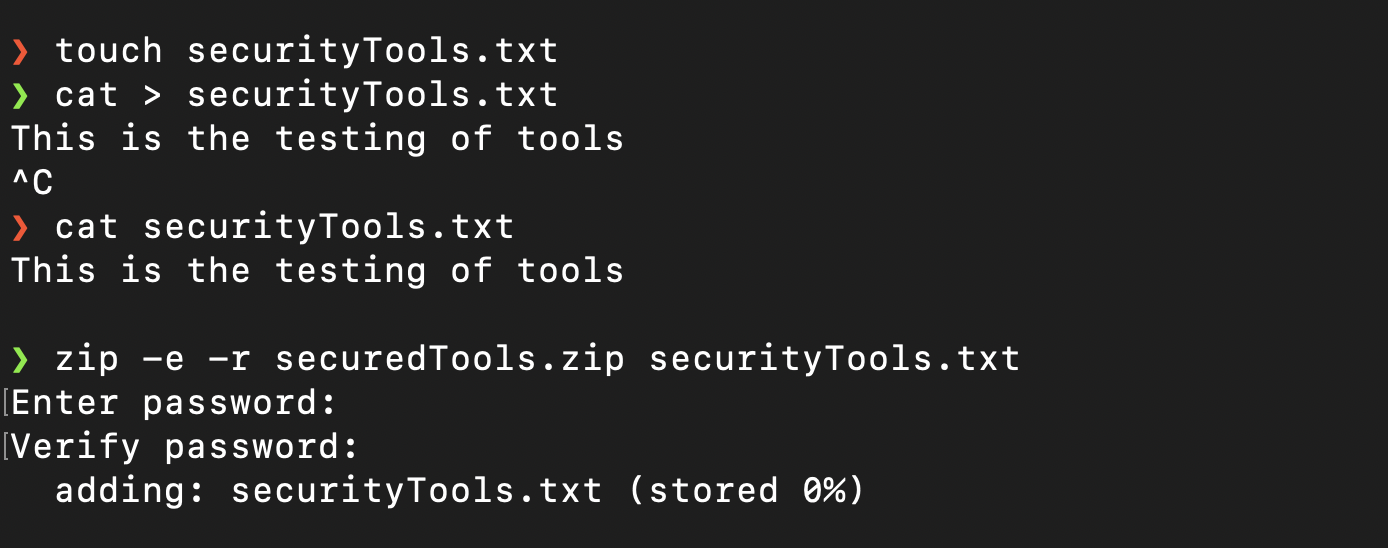
\includegraphics[width=\textwidth]{images/0.png}
        \end{figure}
        \item Create a hashfile of password \\
        \texttt 
        {./zip2john <zip\_file> <hash\_file>}\\ 
         \begin{figure}[H]
            \centering
            
\includegraphics{images/1.png}
        \end{figure}
        \item Crack the file in single mode \\
        \texttt 
        {./john --single <hash\_file>}\\ 
         \begin{figure}[H]
            \centering
            
\includegraphics{images/2.png}
        \end{figure}
        \item Cracking Process \\
         \begin{figure}[H]
            \centering
            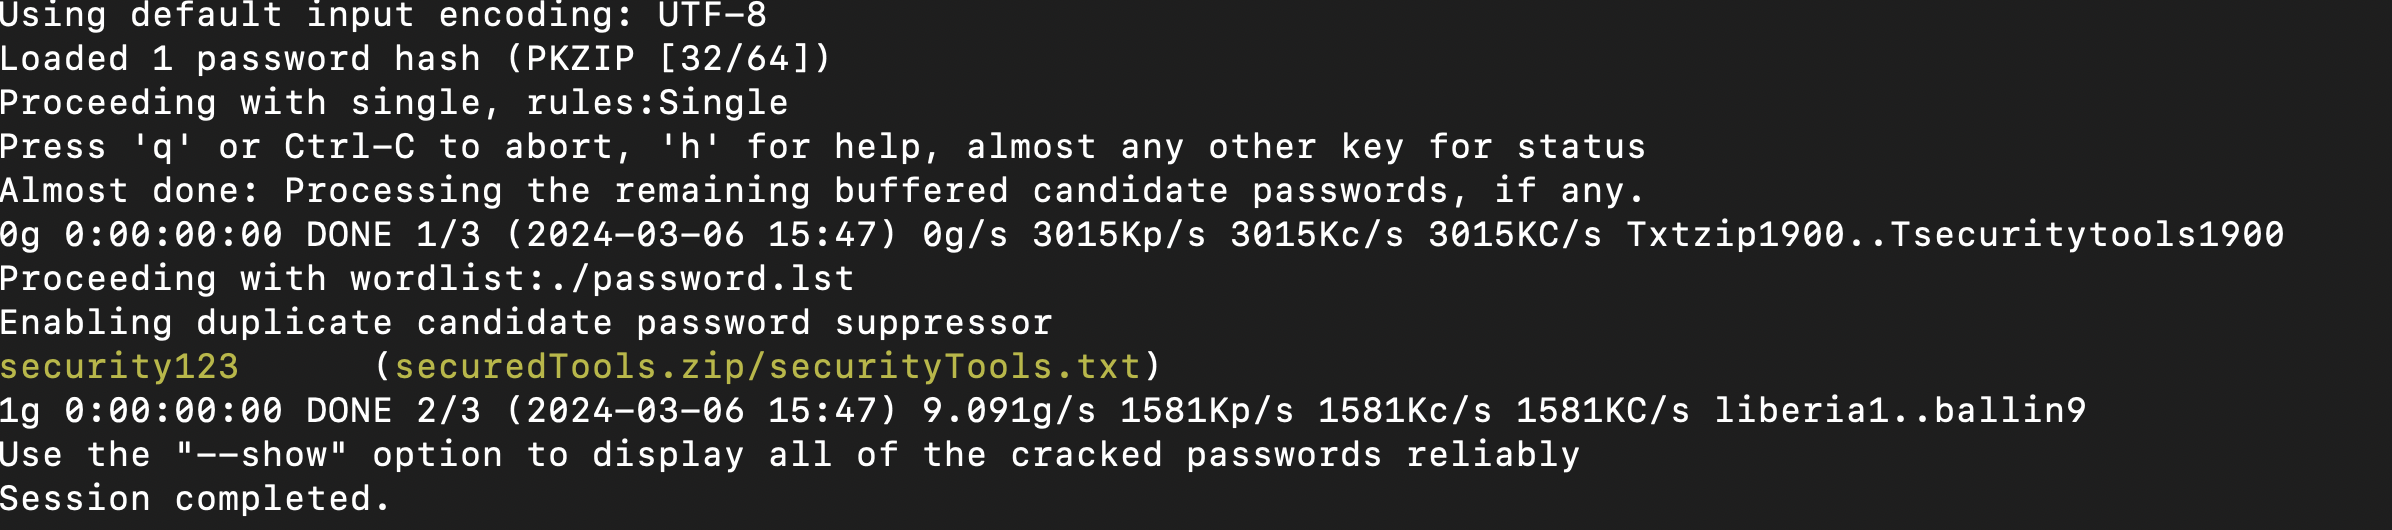
\includegraphics[width=\textwidth]{images/3.png}
        \end{figure}
        \item Show the password \\
         \begin{figure}[H]
            \centering
            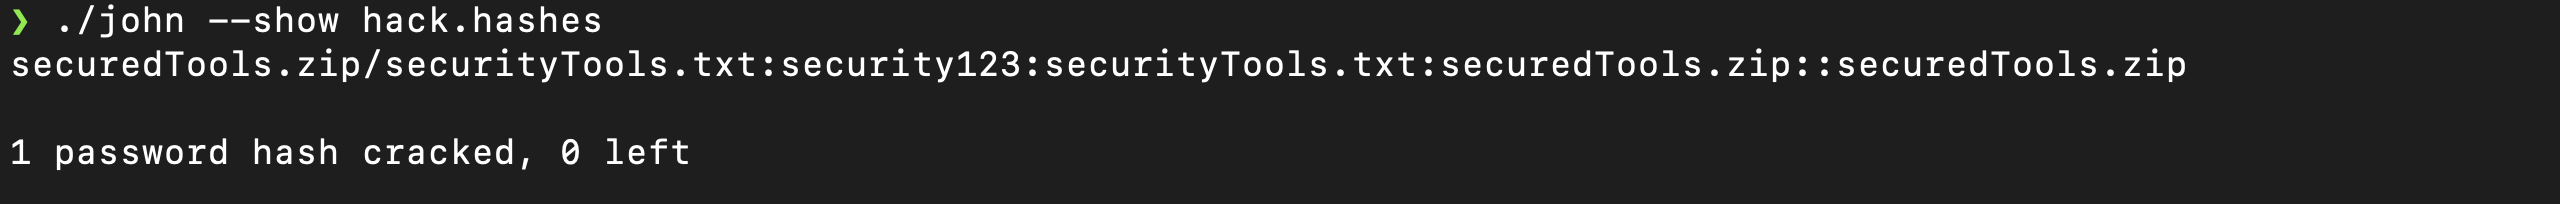
\includegraphics[width=\textwidth]{images/4.png}
        \end{figure}
         \begin{figure}[H]
            \centering
            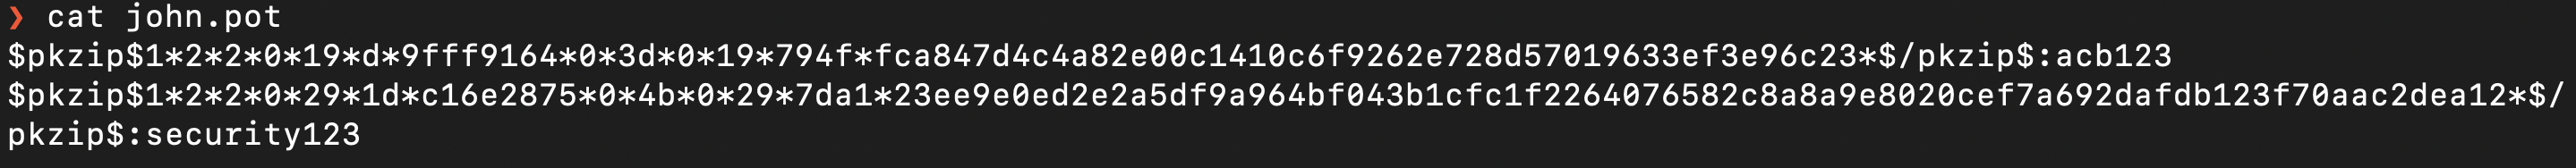
\includegraphics{images/5.png}
        \end{figure}
        \item Unzip and access the file using the password you get \\
        \texttt 
        {./john --single <hash\_file>}\\ 
         \begin{figure}[H]
            \centering
            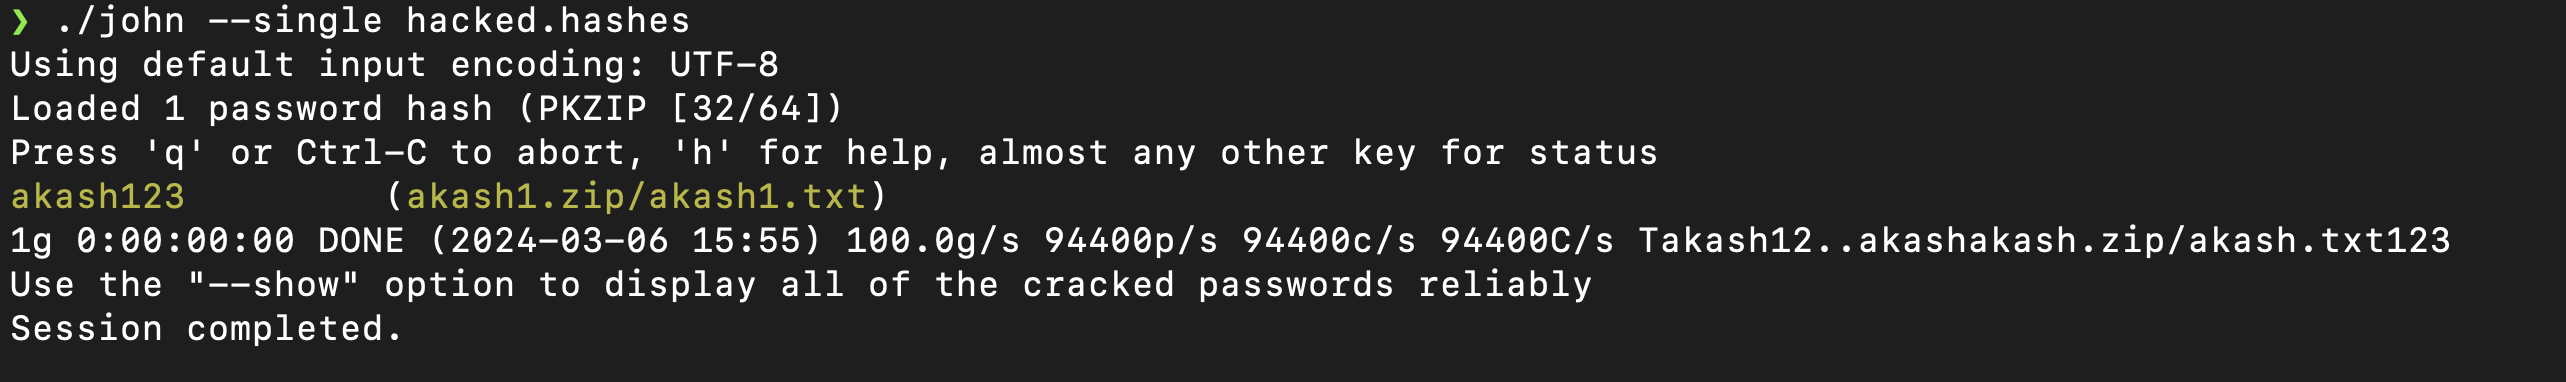
\includegraphics[width=\textwidth]{images/6.png}
        \end{figure}
    \end{itemize}
    \newpage

    
    \item \textbf{\large{Dictionary Attack(Wordlist method):}}
    \begin{itemize}
        \item Create a temporary user to crack his password \\
        \textbf {\textit{sudo adduser cassandra}}\\ 
         \begin{figure}[H]
            \centering
            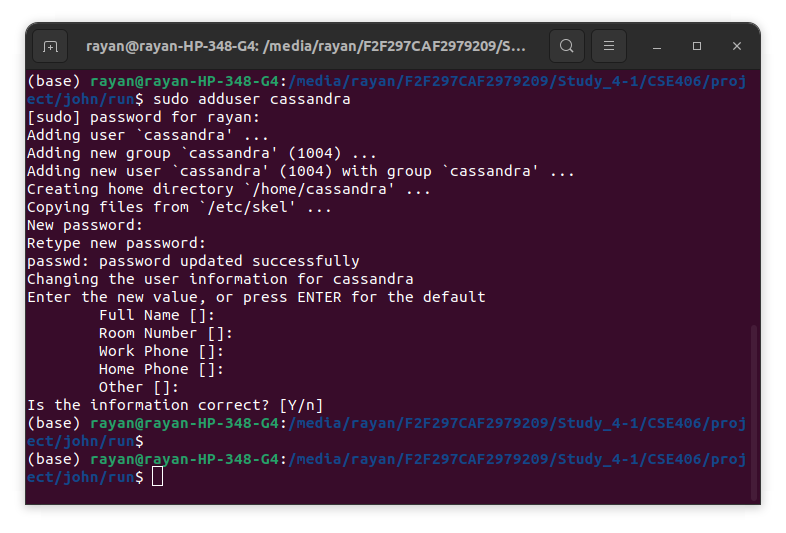
\includegraphics[width=\textwidth]{images/word1.png}
        \end{figure}
         \item Shadow folder has the hashes of passwords. The only access is of root. We have to grep \textbf {\textit{/etc/shadow }} folder to \textbf {\textit{newpass}}. \\
         \begin{figure}[H]
            \centering
            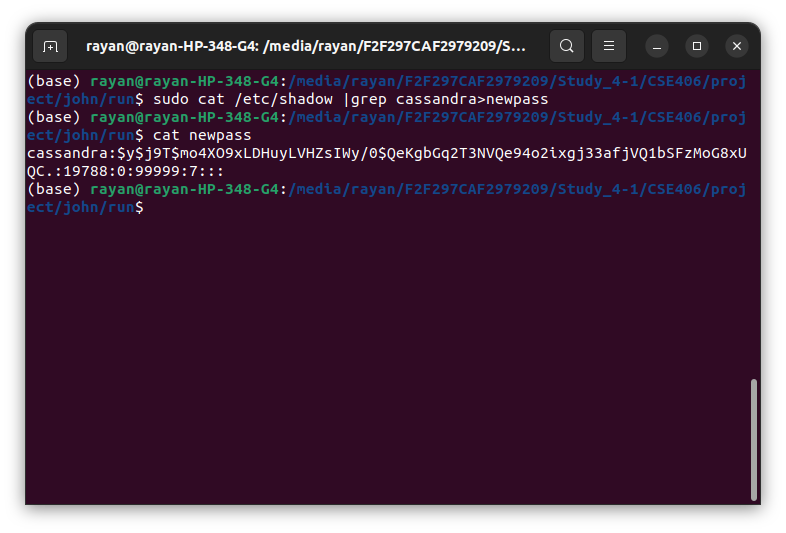
\includegraphics[width=\textwidth]{images/word2.png}
        \end{figure}
        
        \item Default wordlist attack
        \textit{\textbf{./john --wordlist=pospass newpass}}
        \begin{figure}[H]
            \centering
            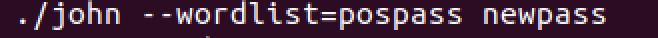
\includegraphics{images/000.png}
        \end{figure}
    \end{itemize}

    \item \textbf{\large{Dictionary Attack(Manual wordlist method):}}
    \begin{itemize}
        \item Create a your own wordlist\\
         \begin{figure}[H]
            \centering
            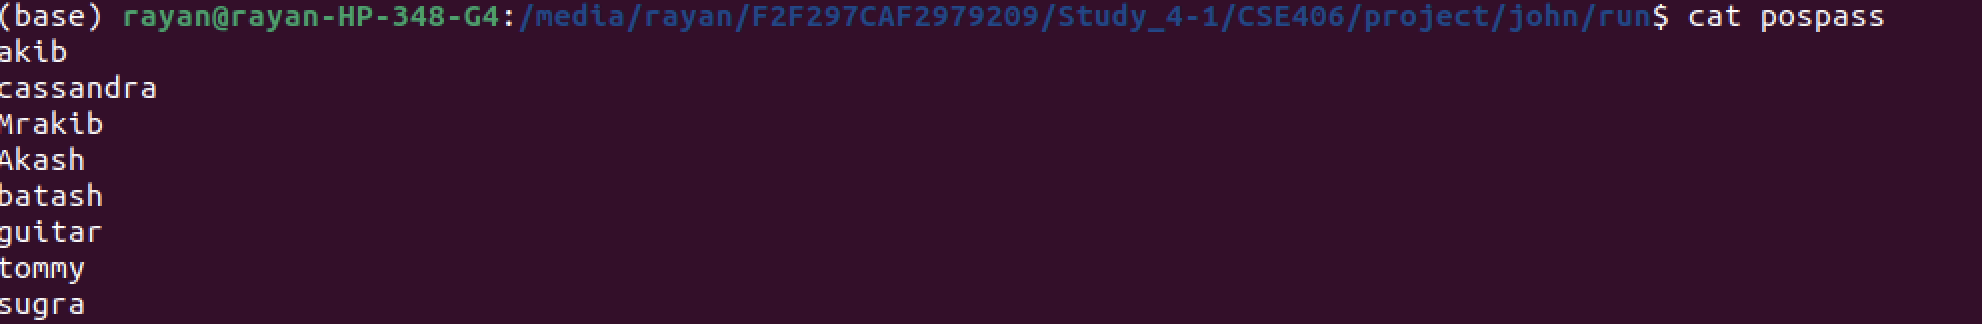
\includegraphics[width=\textwidth]{images/w0.png}
        \end{figure}
         \item Attack with manual wordlist
         \textit{\textbf{./john --wordlist=pospass newpass}}
         \begin{figure}[H]
            \centering
            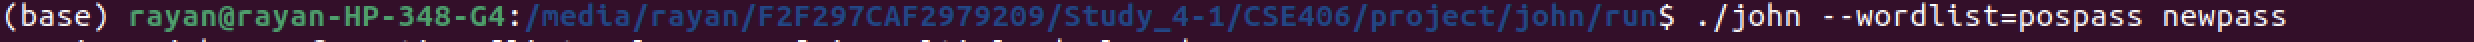
\includegraphics[width=\textwidth]{images/w1.png}
        \end{figure}
        \item Cracking Process
        \begin{figure}[H]
            \centering
            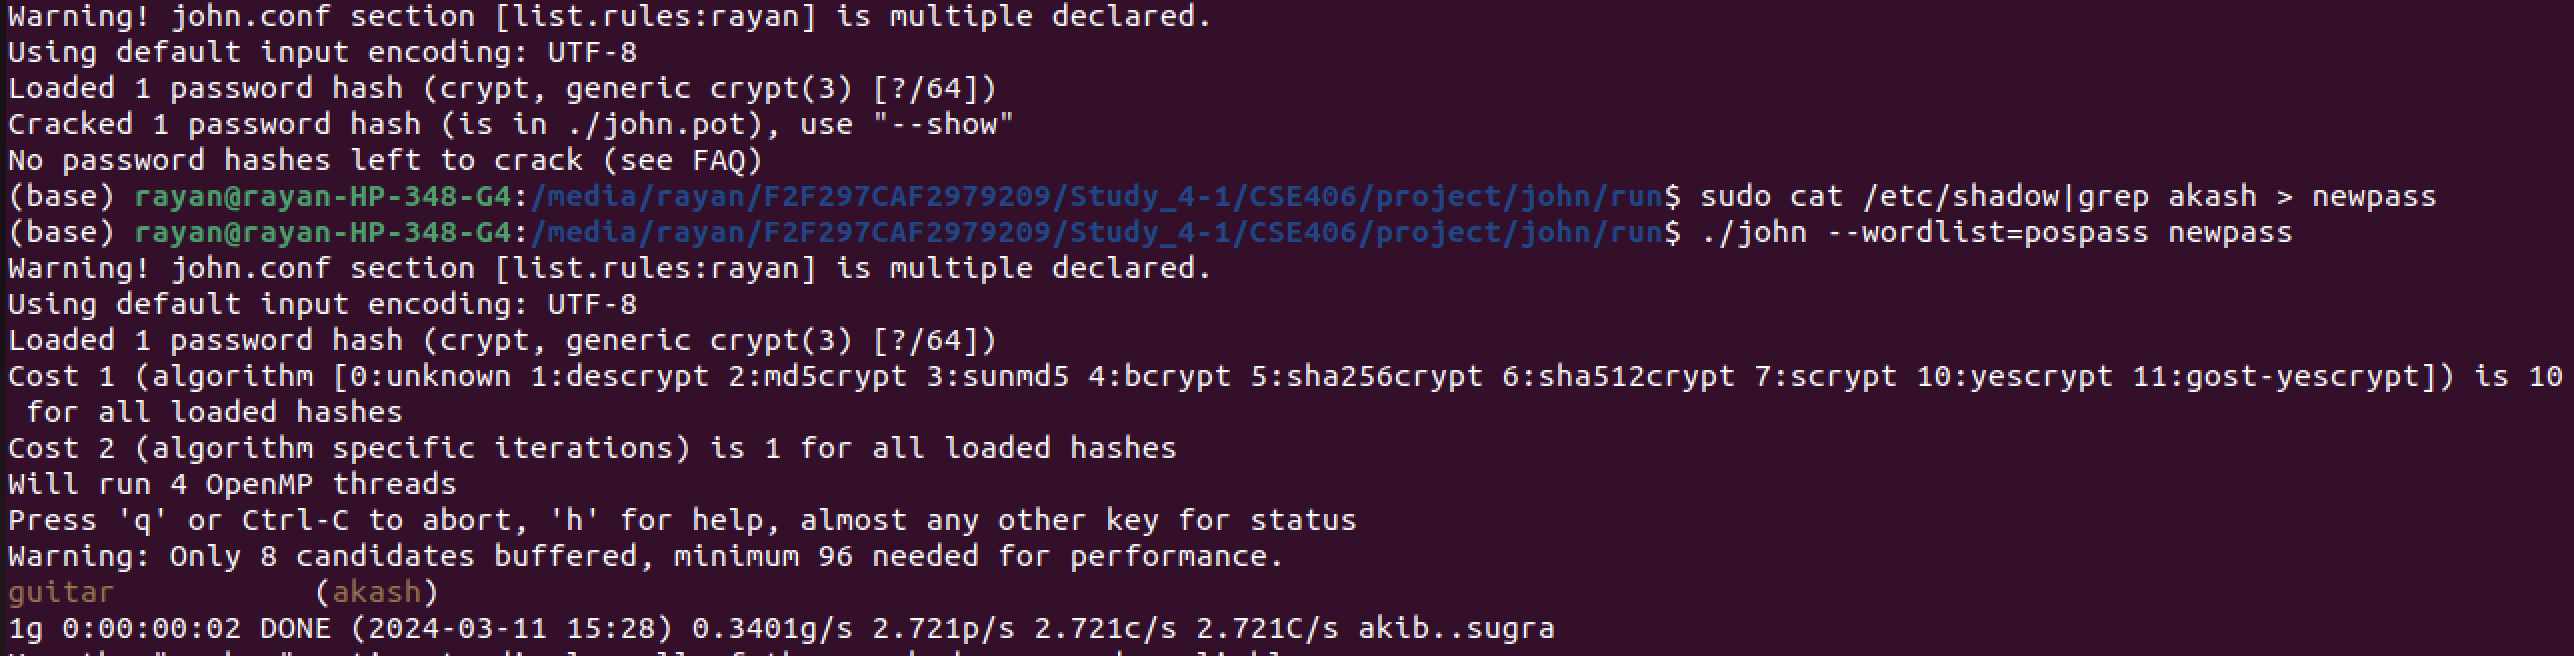
\includegraphics[width=\textwidth]{images/w2.png}
        \end{figure}
    \end{itemize}

    \item \textbf{\large{Dictionary Attack(Rule-Based method):}}
    \begin{itemize}
        \item Create some Rules\\
         \begin{figure}[H]
            \centering
            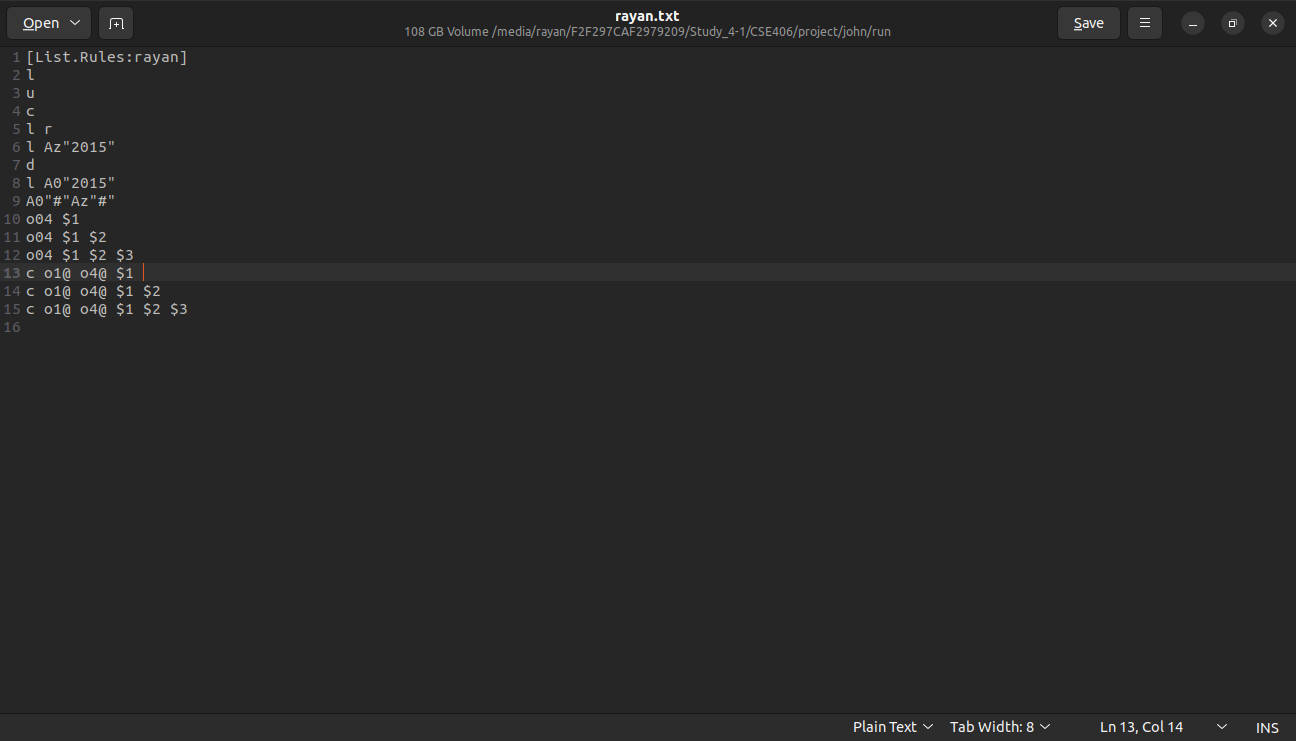
\includegraphics[width=\textwidth]{images/rule0.png}
        \end{figure}
         \item Show the rules
         \textit{\textbf{./john --wordlist=pospass --stdout --rules:rayan}}
         \begin{figure}[H]
            \centering
            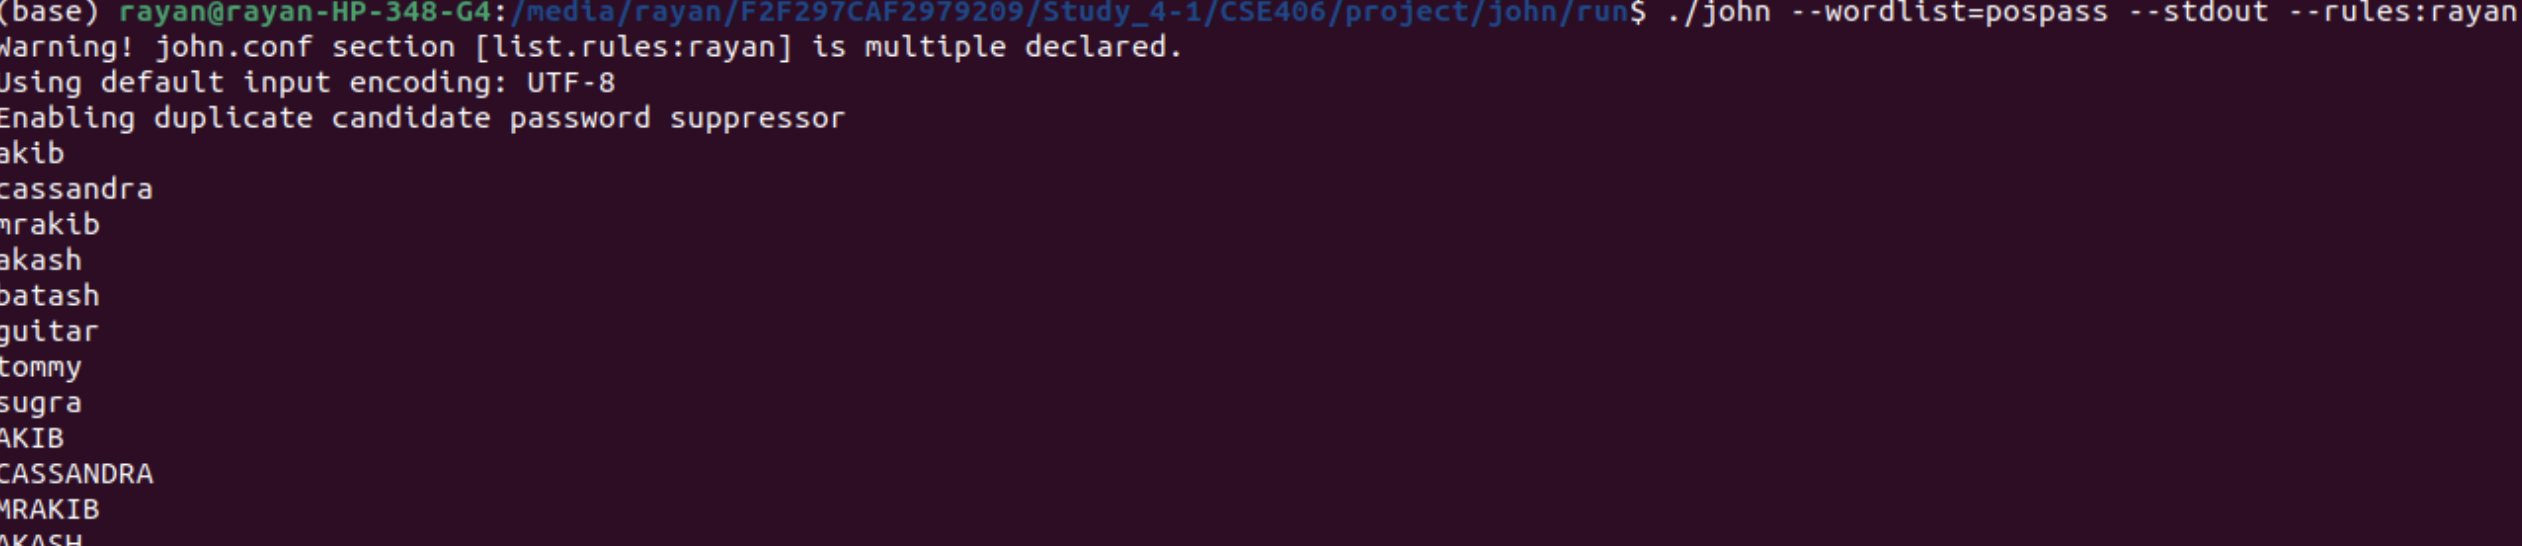
\includegraphics[width=\textwidth]{images/rule9999.png}
        \end{figure}
         \begin{figure}[H]
            \centering
            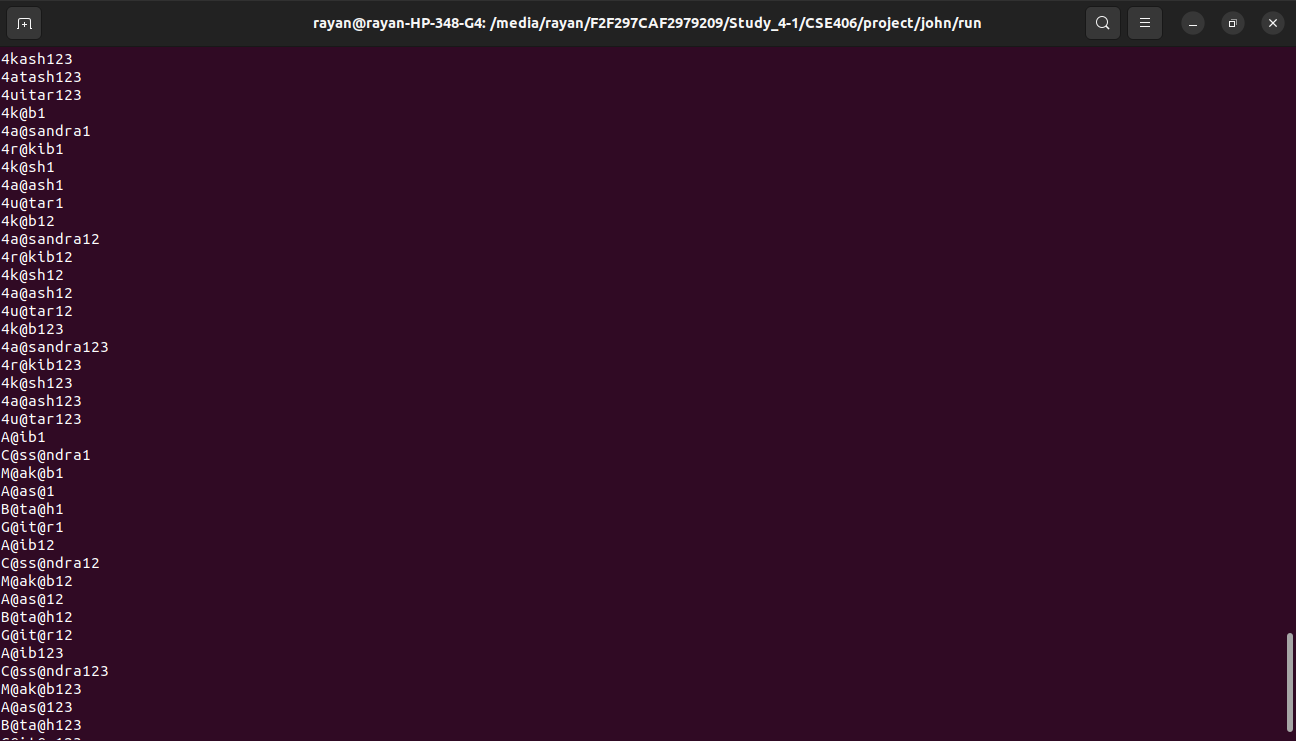
\includegraphics[width=\textwidth]{images/rule11.png}
        \end{figure}
        \item Rule-Based Attack
        \textit{\textbf{./john --wordlist=pospass --rules:rayan}}
        \begin{figure}[H]
            \centering
            
\includegraphics[width=\textwidth]{images/ruleAttack.png}
        \end{figure}
        
        \item Cracking Process
        \begin{figure}[H]
            \centering
            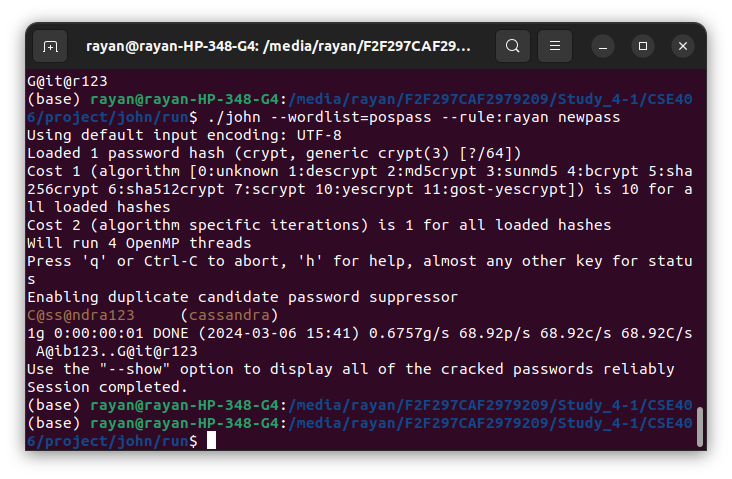
\includegraphics[width=\textwidth]{images/rule2.png}
        \end{figure}
    \end{itemize}
\end{enumerate}
\vspace{0.4cm}

\section{Failures}
Despite its effectiveness, John the Ripper may fail to crack passwords under certain circumstances, such as:

\begin{itemize}
    \item \textbf{Strong Passwords:}  Passwords that are sufficiently complex and long may remain uncrackable by John the Ripper, especially if they are not included in any dictionary or have random character sequences.
    \item \textbf{Salted Hashes:} If the passwords are stored using cryptographic hashing algorithms with salts, it significantly increases the difficulty of cracking them, and John the Ripper may not be successful without additional resources or time.
\end{itemize}
John the Ripper is a valuable tool in the arsenal of security professionals for identifying weak passwords and enhancing the overall security posture of systems and networks. However, it's essential to understand its capabilities, limitations, and proper usage to derive maximum benefit from its features.
\vspace{0.4cm}

\section{Optimization:}
John the ripper can be optimized for better performance -

1. Parallel computation (multiple CPU)
2. Optimised hash (format)
3. Optimised algorithm (adding rules)

\begin{itemize}
    \item \textbf{Parallel computation:} It can distribute the workload across multiple processors, cores, or GPUs to increase speed.  
    \item \textbf{Optimized Hash Functions:} If we can guess what hash function is used in password, we can select respective mode for efficient comparison and performance.
    \item \textbf{Efficient Algorithms:} For brute-force and incremental modes, it employs efficient algorithms to reduce unnecessary computations.
    
\end{itemize}

\vspace{0.4cm}

\end{document}
